\documentclass[12pt]{article}
\usepackage{amsmath}
\usepackage{amssymb}
\usepackage{graphicx}
\usepackage{setspace}
\begin{document}
\title{Matrix Project}
\maketitle
\author{G.Naga Dhanush  EE17BTECH11014\\B.Gowrishankar Reddy   EE17BTECH11009}
\section{problem}
A variable line drawn through the intersection of the lines\\
(4 3)X = 12\\
(3 4)X = 12\\
meets the coordinate axes at A and B, then find the locus of the midpoint of AB.
\section{solution}
The given linear equations are \\
\[
\begin{bmatrix}
 4 & 3 \\
 3 & 4
\end{bmatrix}X = 
\begin{bmatrix}
 12 \\
 12
\end{bmatrix}
\]
 
 \[
Let P = 
\begin{bmatrix}
 4 & 3 \\
 3 & 4
\end{bmatrix},
 Q =
\begin{bmatrix}
 12 \\
 12
\end{bmatrix} 
\]
\begin{center}
PX = Q\\
X = $P^{-1}$Q\\
X is point of intersection

\end{center}
\[
X = 
\begin{bmatrix}
 1.714 \\
 1.714
\end{bmatrix}
\]
Variable line passing through X is
\[ 
\begin{bmatrix}
 m & -1
\end{bmatrix}X = 1.714(m-1)
\]
where m is parameter for variable line\\
It meets cordinate axes at A and B respectively.\\

\[
A = 
\begin{bmatrix}
 a \\
 0
\end{bmatrix}
B = 
\begin{bmatrix}
 0 \\
 b
\end{bmatrix}
\]
a = 1.714$\frac{(m-1)}{m}$,b = 1.714(1-m)
The locus of midpoint of A and B is C
\[
C = 
\begin{bmatrix}
 x \\
 y
\end{bmatrix}
\]
\begin{center}
x,y are a/2 and b/2 respectively\\
\singlespacing
x =$\frac{0.8571(m-1)}{m}$, y = 0.8571(1-m)\\
\singlespacing
y/x = m\\
\singlespacing
y = 0.8571(1-$\frac{y}{x}$)\\
\singlespacing
xy = 0.8571(x-y)\\
\singlespacing
Therefore the locus is a hyperbola whose equation is
\[
C = 
\begin{bmatrix}
  0.8571(m-1)/m \\
  0.8571(1-m)
\end{bmatrix}
\]
m is paramter.

\begin{figure}[h]
\begin{center}
\textbf{FIGURES}\\
\end{center}
{The figure of this locus obtained from python code}
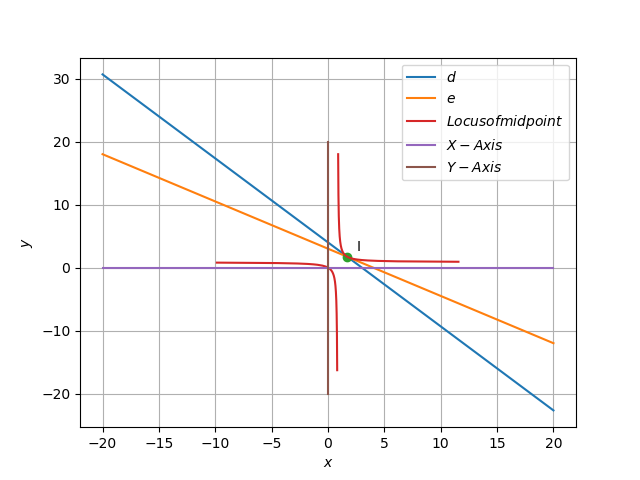
\includegraphics[scale=0.75]{locus}
\caption{locus diagram}
The figure of variable lines passing through X
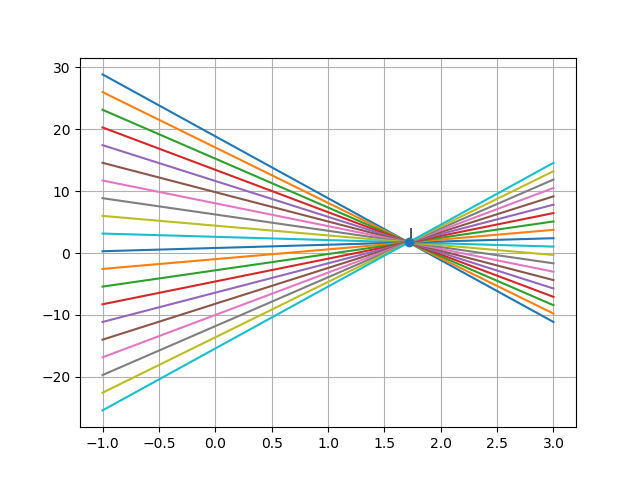
\includegraphics[scale=0.75]{variable_lines}
\end{figure}
\end{center}
\end{document}